\documentclass[12pt,a4paper]{scrartcl}
\usepackage[utf8]{inputenc}
\usepackage[english,russian]{babel}
\usepackage{indentfirst}
\usepackage{misccorr}
\usepackage{graphicx}
\usepackage{amsmath}
\usepackage{multirow}
\usepackage{pgfplots}
\usepackage[top=1cm, bottom=1cm, left=1cm, right=1cm]{geometry}
\pgfplotsset{compat=1.9}

\begin{document}
	\graphicspath{{C:/Users/Alex/OneDrive/Изображения/TexImgs}}
	
	\newcommand{\ms}{\mathstrut}
	\newcommand{\msp}{\hspace{0.5cm}}
	\newcommand{\al}{\alpha}
	\newcommand{\dg}{^\circ}
	\newcommand{\qd}[2]{^{\frac{#1}{#2}}}
	\newcommand{\qdm}[2]{^{-\frac{#1}{#2}}}
	\newcommand{\lm}[2]{\underset{#1 \rightarrow #2}{\lim}}
	\newcommand{\sfrac}[2]{\dfrac{\strut #1}{\strut #2}}
	\newcommand{\equal}[1]{\overset{(#1)}{=}}
	\newcommand{\linevdots}{\ \raisebox{-.08\height}{\vdots}\ }
	\newcommand{\linecvdots}{\ \raisebox{-.08\height}{\vdots}\hspace{-0.13cm}\raisebox{.15\height}{\cancel{\phantom{a}}\hspace{0.06cm}}}
	\newcommand{\combox}[1]{\ms \msp \msp \begin{minipage}{0.95\linewidth}
			#1
	\end{minipage}}
	
	\newtheorem{pr}{Задача}
	\newtheorem{ex}{Пример}
	
	\newenvironment{slv}{\ms \msp \textit{Решение:}}{}
	\newenvironment{proof}{\ms \msp \textit{Доказательство: }}{\hfill $\square$}
	
	\begin{titlepage}
		
		\vspace*{\fill}
		
		\begin{center}
			
\includegraphics[scale=0.8]{MIPT.png}
			\\[0.7cm]\Huge Московский Физико-Технический Институт\\(национальный исследовательский университет)
			\\[2cm]\LARGE Отчет по эксперименту
			\\[0.5cm]\noindent\rule{\textwidth}{1pt}
			\\\Huge\textbf{Измерение удельного сопротивления\\нихромовой проволоки}
			\\[-0.5cm]\noindent\rule{\textwidth}{1pt}
		\end{center}
		
		\begin{flushleft}
			\textit{Работа №1.1.1; дата: 20.09.21}\hfill\textit{Семестр: 1}
		\end{flushleft}
		
		\vspace*{\fill}
		
		\begin{flushleft}
			Выполнил: \hspace{\fill} Группа:
			\\Кошелев Александр \hspace{\fill} Б05-105
		\end{flushleft}
	\end{titlepage}
	
	%Страница 2
	
	\begin{flushleft}
		\footnotesize{Измерение удельного сопротивления нихромовой проволоки} \hspace{\fill} \footnotesize{2}
		\\[-0.3cm]\noindent\rule{\textwidth}{0.3pt}
	\end{flushleft}

	\section{Аннотация}
	В работе измеряется удельное сопротивление тонкой проволоки круглого сечения, изготовленной из нихромового сплава. Используются следующие методы измерения сопротивления:
	\begin{enumerate}
		\item Определение углового коэффициента наклона зависимости напряжения на проволоке от тока
		через неё, измеряемых с помощью аналоговых и цифровых вольтметров и амперметров.
		\item Измерение с помощью моста постоянного тока.
	\end{enumerate}
	 Геометрические размеры образца измеряются с
	помощью линейки, штангенциркуля и микрометра. Детально исследуются систематические и случайные погрешности проводимых измерений. 
	
	\section{Теоретические сведения}
	Пусть $R$ --- сопротивление проволоки, $d$ --- диаметр, $l$ --- длина, тогда удельное сопротивление ее материала $\rho$ может быть найдено как: 
	\begin{equation}
		\rho = R\sfrac{\pi d^2}{4l}
	\end{equation}

	В соответствии с законом Ома сила тока $I$ и напряжение $U$ в образце связаны через сопротивление $R$ образца как:
	\begin{equation}
		U = IR	
	\end{equation} 

	Для измерения напряжения и силы тока использовалась схема, представленная на рис. 1. 
	\begin{center}
		\includegraphics*[scale=0.2]{PIC_1.png}
		\\\textbf{Рис. 1:} Схема экспериментальной установки
	\end{center}

	Поскольку использованный в работе вольтметр неидеальный, необходимо учесть его внутреннее сопротивление. Обозначим его $R_V$, показания вольтметра $U_V$, а показания амперметра --- $I_A$. С помощью закона Ома их можно связать соотношением
	\begin{equation}
		U_V = I_A R'
	\end{equation}
	где $R'$ - сопротивление параллельно соединенных вольтметра и образца, которое может быть найдено по формуле
	\begin{equation}
		\sfrac{1}{R'} = \sfrac{1}{R} + \sfrac{1}{R_V}
	\end{equation}
	Принимая во внимание, что $R_V \gg R,  R'$, в соответствии с формулой (3) график $U_V(I_A)$ --- прямая с коэффициентом наклона $R'$, откуда можно найти сопротивление как:
	\begin{equation}
		R = \sfrac{R_V R'}{R_V - R'} \approx R'\left(1 + \sfrac{R'}{R_V}\right)
	\end{equation}

	\newpage
	\begin{flushleft}
		\footnotesize{Измерение удельного сопротивления нихромовой проволоки} \hspace{\fill} \footnotesize{3}
		\\[-0.3cm]\noindent\rule{\textwidth}{0.3pt}
	\end{flushleft}
	

	\section{Оборудование и инструментальные погрешности}
	
	\paragraph{Линейка} \hfill
	
	\par $\Delta_{\text{лин}} = \pm0.5\,$мм (из цены деления). При определении расстояния между контактами возможна дополнительная случайная погрешность, которую можно оценить как $\Delta_{\text{лин}} = \pm2\,$мм.
	
	\paragraph{Штангенциркуль} \hfill
	
	\par $\Delta_{\text{шц}} = \pm 0.05\,$мм (по маркировке производителя).
	
	\paragraph{Микрометр} \hfill
	
	\par $\Delta_{\text{мкм}} = \pm 0.01\,$мм (по маркировке производителя).
	
	\paragraph{Вольтметр} \hfill
	\begin{center}
		\begin{tabular}{|c|c|c|}
			\hline Система & \multicolumn{2}{|c|}{Магнито-электрическая}
			\\\hline Класс точности & \multicolumn{2}{|c|}{0.5}
			\\\hline Шкала & \multicolumn{2}{|c|}{Линейная, 150 делений}
			\\\hline Предел измерений & $0.75\,$В & $1.5\,$В
			\\\hline Цена деления & $5\,$мВ & $10\,$мВ
			\\\hline Чувствительность & $200\,$дел./В & $150\,$дел./В
			\\\hline Внутреннее сопротивление & $R_V = 5\,$кОм & $R_V = 10\,$кОм
			\\\hline Погрешность при считывании & \multirow{2}{*}{$\pm 2.5\,$мВ} & \multirow{2}{*}{$\pm 5\,$мВ}
			\\ со шкалы (0.5 шкалы деления) &&
			\\\hline Макс. погрешность & \multirow{2}{*}{$\pm 3.75\,$мВ (0.5\%)} & \multirow{2}{*}{$\pm 7.5\,$мВ (0.5\%)}
			\\ согласно классу точности &&
			\\\hline
		\end{tabular}
		\\\textbf{Табл. 1:} Характеристики вольтметра
	\end{center}

	\paragraph{Амперметр} \hfill
	
	\begin{center}
		\begin{tabular}{|c|c|}
			\hline Система & Цифровая
			\\\hline Предел измерений & $2\,$А
			\\\hline Разрядность дисплея & $5\,$ед.
			\\\hline Внутреннее сопротивление & $R_A = 1.4\,$Ом
			\\\hline Погрешность & $\Delta_A = \pm(0.002 \cdot X + 2k)$
			\\ (при комнатной температуре, & \multicolumn{1}{|l|}{где $X$ --- измеряемая величина,}
			\\ согласно паспорту) & \multicolumn{1}{|l|}{$k$ --- единица младшего разряда ($0.01\,$мА)}
			\\\hline
		\end{tabular}
		\\\textbf{Табл. 2:} Характеристики амперметра
	\end{center}
	\vspace{-0.3cm}При измерениях в диапазоне от $20\,$мА до $300\,$мА погрешность амперметра составила соответственно от $\Delta_A = \pm 0.06\,$мА (0.3\%) до $\Delta_A = \pm 0.6\,$мА (0.2\%)
	
	\medskip В диапазоне измерения $R$ от 1 до 10$\,$Ом относительная поправка $\frac{R'}{R_V}$ к сопротивлению согласно ф-ле (5) составляет от 0.01\% (при $R = 1\,$Ом и $R_V = 10$кОм) до 0,2\% (при $R = 10\,$Ом и
	$R_V = 5\,$кОм). Следовательно, данная поправка заведомо меньше погрешности измерений (0.5\% для вольтметра), поэтому примем далее, что неидеальность амперметра не оказывает влияния на измерение сопротивления:
	\begin{equation}
		R \approx R_V
	\end{equation}

	\paragraph{Мост постоянного тока Р4833} \hfill
	\begin{center}
		\begin{tabular}{|c|c|}
			\hline Класс точности & 0.1
			\\\hline Разрядность магазина сопротивлений & 5$\,$ед
			\\\hline Используемый диапазон измерений & $10^{-4} - 10\,$Ом
			\\\hline Погрешность в диапазоне & $\pm0.010\,$Ом
			\\\hline
		\end{tabular}
		\\\textbf{Табл. 3:} Характеристики моста
	\end{center}
	
	\newpage
	\begin{flushleft}
		\footnotesize{Измерение удельного сопротивления нихромовой проволоки} \hspace{\fill} \footnotesize{4}
		\\[-0.3cm]\noindent\rule{\textwidth}{0.3pt}
	\end{flushleft}
	
	\section{Измерения и обработка данных}
	
	
	\paragraph{4.1 Измерение диаметра проволоки} \hfill
	\par Измерения диаметра проволоки проводились на разных ее участках при помощи штангенциркуля и микрометра. При измерении диаметра штангенциркулем при $N = 10$ измерениях получены одинаковые значения $d = 0.35\,$мм. При измерении микрометром показания не были одинаковыми, занесем их в таблицу:
	\begin{center}
		\begin{tabular}{|c|c|c|c|c|c|c|c|c|c|c|}
			\hline $i,$ номер & 1 & 2 & 3 & 4 & 5 & 6 & 7 & 8 & 9 & 10
			\\\hline $d_i,\,$мм & 0.37 & 0.365 & 0.37 & 0.36 & 0.365 & 0.36 & 0.36 & 0.35 & 0.355 & 0.355
			\\\hline 
		\end{tabular}
		\\\textbf{Табл. 4:} Измерение диаметра проволоки микрометром 
	\end{center}
	
	Среднее значение диаметра: $\overline{d} = \sfrac{\overset{N}{\underset{i = 1}{\sum}} d_i}{N} = 0.361\,$мм
	\par Стандартное отклонение: $\sigma_d = \sqrt{\sfrac{1}{N-1}\overset{N}{\underset{i = 1}{\sum}} (\overline{d} - d_i)^2} \approx 0.0066\,$мм
	\par Случайная погрешность среднего: $\sigma_{\overline{d}} = \sfrac{\sigma_d}{\sqrt{N}} \approx 0.0021\,$мм
	\par С учетом инструментальной погрешности $\Delta_{\text{мкм}} = 0.01\,$мм погрешность измерения диаметра может быть вычислена как:
	$$\sigma_{\overline{d}}^{\text{полн}} = \sqrt{\sigma_{\overline{d}}^2 + \Delta_{\text{мкм}}^2} \approx 0.0102\,\text{мм}$$

	\textit{Окончательные результаты измерения диаметра проволоки:}
	\par \textit{Штангенциркулем:} $d = (0.35 \pm 0.05)\,$мм
	\par \textit{Микрометром:} $d = (0.361 \pm 0.010)\,$мм (при $\varepsilon_d = 3.1\%$)

	\paragraph{4.2 Измерение сопротивления проволоки} \hfill

	\par Результаты измерений зависимости показаний вольтметра $U_V$ от показаний амперметра $I_A$ запишем в таблицу 5 и построим по ним графики зависимости $U_V(I_A)$, пользуясь методом наименьших квадратов (Рис. 2, 3). Причем для $l = 50\,$см измерения проведем с изменением полярности.
	\par Получившиеся графики представляют из себя в пределах погрешности прямые, проходящие из начала координат, что подтверждает теоретический прогноз формулы (3).
	\begin{center}
		\begin{tabular}{|c|c|c|c|c|c|c|}
			\hline \multicolumn{7}{|c|}{$l = (50.0 \pm 0.2)\,$см} 			\\\hline $U_V,\,$мВ & 300 & 335 & 370 & 405 & 440 & 475 
			\\\hline $I_A,\,$мА & 60.61 & 67.93 & 75.10 & 82.16 & 89.61 & 96.34 
			\\\hline $I_A,\,$мА & 60.79 & 68.08 & 75.02 & 82.16 & 89.42 & 96.65
			\\\hline $U_V,\,$мВ & 510 & 545 & 580 & 615 & 650 & 685
			\\\hline $I_A,\,$мА & 103.36 & 110.61 & 117.40 & 124.42 & 131.63 & 138.80
			\\\hline $I_A,\,$мА & 103.37 & 110.55 & 117.57 & 124.60 & 131.63 & 138.80
			\\\hline \multicolumn{7}{|c|}{$l = (30.0 \pm 0.2)\,$см}
			\\\hline $U_V,\,$мВ & 300 & 335 & 370 & 405 & 440 & 475 
			\\\hline $I_A,\,$мА & 100.15 & 111.71 & 123.71 & 135.78 & 147.16 & 158.94 
			\\\hline $U_V,\,$мВ & 510 & 545 & 580 & 615 & 650 & 685
			\\\hline $I_A,\,$мА & 170.52 & 182.10 & 193.81 & 205.43 & 216.93 & 228.48
			\\\hline
		\end{tabular}
		\\\textbf{Табл. 5:} Зависимость $U_V$ от $I_A$
	\end{center}

	Заметим, что при изменении полярности получаем зависимость напряжения от силы тока очень близкую к изначальной. Отклонения происходят только в нескольких точках из всего набора измерений.
	
	\newpage
	\begin{flushleft}
		\footnotesize{Измерение удельного сопротивления нихромовой проволоки} \hspace{\fill} \footnotesize{5}
		\\[-0.3cm]\noindent\rule{\textwidth}{0.3pt}
	\end{flushleft}

	\begin{center}
		\begin{figure}[h]
			\begin{minipage}{0.5\linewidth}
				\begin{center}
					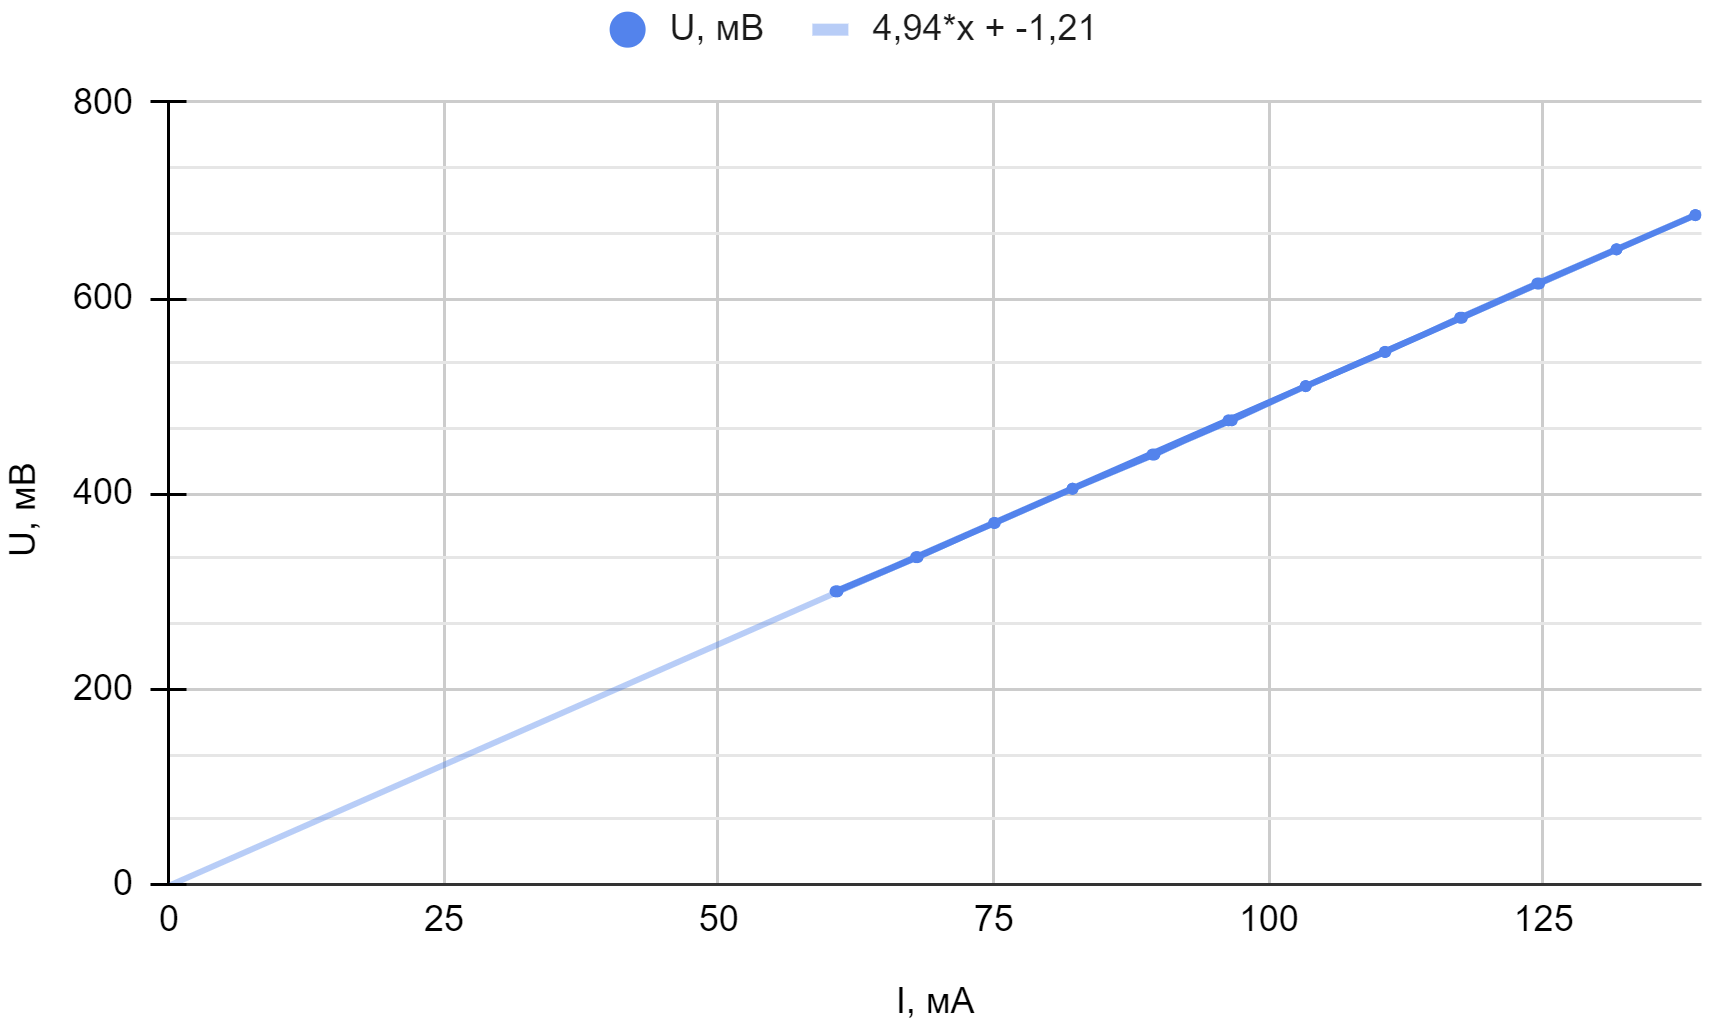
\includegraphics[scale=0.2]{PIC_2.png}
					\\\textbf{Рис. 2:} График $U_V(I_A),\ l = (50.0 \pm 0.2)\,$см
				\end{center}
			\end{minipage}
			\begin{minipage}{0.5\linewidth}
				\begin{center}
					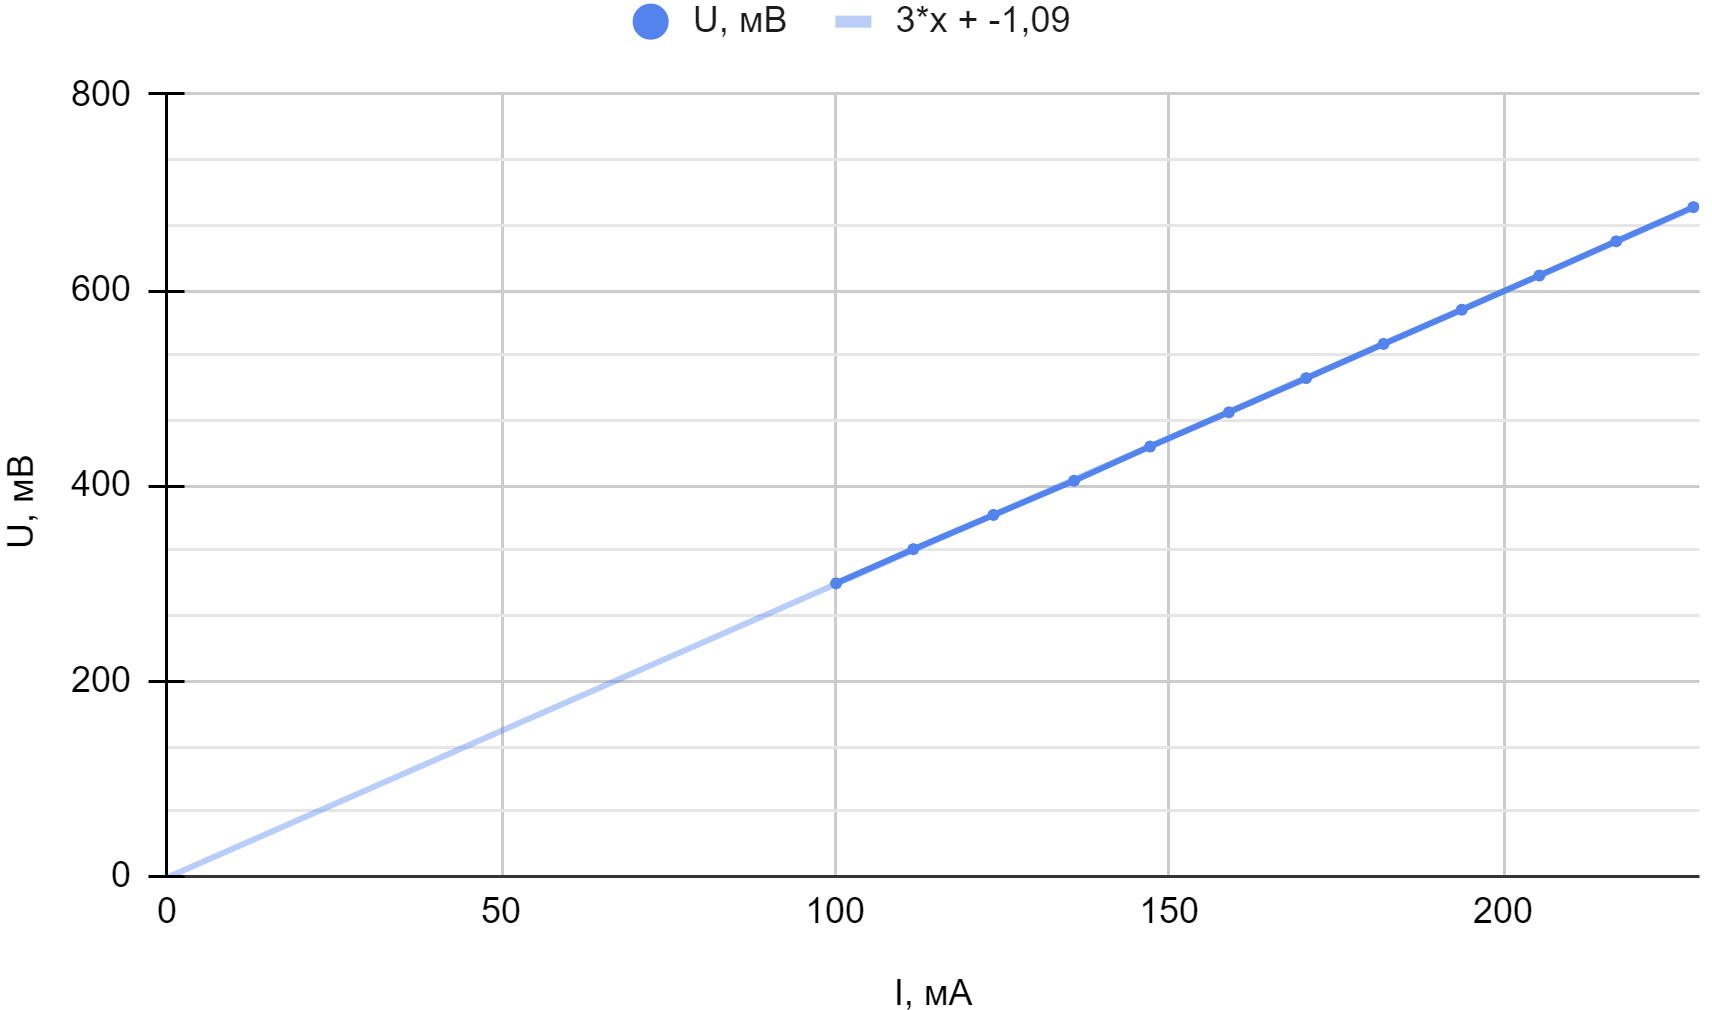
\includegraphics[scale=0.201]{PIC_3.png}
					\\\textbf{Рис. 3:} График $U_V(I_A),\ l = (30.0 \pm 0.2)\,$см
				\end{center}
			\end{minipage}
		\end{figure}
	\end{center}

	Начнем оценивать погрешности. Случайную ошибку определения углового коэффициента рассчитаем по формуле, известной из статистики:
	\begin{equation}
		\sigma_R^{\text{сл}} = \sqrt{\sfrac{1}{N-1}\overset{N}{\underset{i = 1}{\sum}}\left(\sfrac{U_{V\,i}}{I_{A\,i}} - \overline{R}\right)^2}
	\end{equation}
	
	Также необходимо оценить и систематическую погрешность эксперимента. Это можно приблизительно оценить погрешностью при максимальных значениях $U$ и $I$, поскольку погрешность приборов зависит от величины измеряемого значения и близка к постоянной.
	\begin{equation}
		\Delta_{R}^{\text{сист}} = R\sqrt{\left(\sfrac{\Delta_U}{U_{max}}\right)^2 + \left(\sfrac{\Delta_I}{I_{max}}\right)^2}
	\end{equation}

	Таким образом, полная погрешность измерения углового коэффициента:
	\begin{equation}
		\sigma_R = \sqrt{\left(\sigma_R^{\text{сл}}\right)^2 + \left(\Delta_{R}^{\text{сист}}\right)^2}
	\end{equation}

	Результат вместе с погрешностями внесем в единую табл. 6, добавив данные, полученные при помощи моста.
	\begin{center}
		\begin{tabular}{|c|c|c|c|c|c|}
			\hline $l,\,$см & $\overline{R},\,$Ом & $\sigma_R^{\text{сл}},\,$Ом & $\Delta_{R}^{\text{сист}},\,$Ом & $\sigma_R,\,$Ом & $R_{\text{мост}},\,$Ом 
			\\\hline $50.0 \pm 0.2$ & 4.940 & 0.012 & 0.021 & 0.024 & $5.123 \pm 0.010$
			\\\hline $30.0 \pm 0.2$ & 3.000 & 0.009 & 0.013 & 0.015 & $3.177 \pm 0.010$
			\\\hline
		\end{tabular}
		\\\textbf{Табл. 6:} Результаты измерения сопротивления
	\end{center}

	Из данной таблицы видно, что величина случайной ошибки измерения сопротивления меньше систематической погрешности, которая вносит основной вклад в итоговую погрешность. Можно отметить, что результат измерений существенно отличается от контрольного значения, полученного при помощи измерительного моста.

	\newpage
	\begin{flushleft}
		\footnotesize{Измерение удельного сопротивления нихромовой проволоки} \hspace{\fill} \footnotesize{6}
		\\[-0.3cm]\noindent\rule{\textwidth}{0.3pt}
	\end{flushleft}

	\paragraph{4.3 Вычисление удельного сопротивления} \hfill
	\par Воспользуемся формулой (1) для вычисления удельного сопротивления материала проволоки. В качестве полного сопротивления используем значения $\overline{R}$, полученные в пункте 4.2. Также отметим, что в сравнении с погрешностью, вносимой измерением диаметра, остальные малы, поэтому ими можно пренебречь при получении конечного результата. Оформим таблицу.
	
	\begin{center}
		\begin{tabular}{|c|c|}
			\hline $n$, номер опыта & $\rho,\, 10^{-6}\ $Ом$\,\cdot\,$м
			\\\hline 1 & $1.011 \pm 0.057$
			\\\hline 2 & $1.023 \pm 0.058$ 
			\\\hline
		\end{tabular}
	\end{center}
	
	Наконец, усредним полученные значения и получим результат эксперимента:
	$$\overline{\rho} = (1.02 \pm 0.06) \cdot 10^{-6}\ \text{Ом} \cdot \text{м}\ (\varepsilon_\rho = 6.7\%)$$

	\section{Итоги эксперимента}
	Итоговое значение удельного сопротивления определено с относительной погрешностью в 6.7\%. Табличное значение удельного сопротивления нихрома лежит в диапазоне $\rho_{\text{табл}} = (0.97 - 1.14) \cdot 10^{-6}\ \text{Ом} \cdot \text{м}$, что соответствует полученному значению $\rho = (1.02 \pm 0.06) \cdot 10^{-6}\ \text{Ом} \cdot \text{м}$ в пределах одного стандартного отклонения.
	\par Отдельно обратим внимание на то, что измеренное значение сопротивления $R$ не сошлось с результатом, полученным при помощи измерительного моста, являющегося более точным. Причиной этого считаю нестабильную работу моста и возможные неплотные контакты в измерительных схемах. Однако достигнута довольно высокая точность измерений (0.5\%), основная часть погрешности при этом объясняется использованием аналогового вольтметра.
	\par Точность измерения диаметра проволоки также высока засчет использования микрометра. При этом значение случайной ошибки оказалось меньше цены деления микрометра, поэтому уточнение результата с помощью увеличения количества измерений невозможно, как не проверить и однородность диаметра проволоки, что также значительно влияет на ее сопротивление.
	\par Таким образом, для уточнения результата наилучший способ - использование цифрового вольтметра, что позволило бы убрать случайную ошибку при чтении шкалы, и улучшило бы общую точность измерений, так как класс точности цифровых вольтметров выше.
\end{document}